\section{State of the Art}\label{sec:state_of_art}

%----------------------------------------------------------------------

\subsection{Deep Learning Interpretability Techniques}
The current techniques for interpretability or token-level relevance to provide insight and attempt to explain the functioning of transformer architectures in question answering tasks can be divided into three categories:

\subsubsection{Self Attention Mechanisms} 

The self-attention mechanism (\cite{bahdanau2014neural}) in Transformers assigns a pairwise score capturing the relative importance between every two tokens or image patches as attention weights. Thus, a common practice is to use these attention weights to explain the Transformer model’s output by exhibiting the importance distribution over the input tokens (\cite{clark2019does}). The baseline method, RawAtt, utilizes the raw attention weights from a single layer or a combination of multiple layers (\cite{kovaleva2019revealing}). However, recent studies (\cite{serrano2019attention}, \cite{jain2019attention}, \cite{abnar2020quantifying}) question whether highly attentive inputs significantly impact the model outputs. \cite{serrano2019attention} demonstrate that erasing the representations accorded high
attention weights do not necessarily lead to a performance decrease. \cite{jain2019attention} suggest that
“attention is not explanation” by observing that attention scores are frequently inconsistent with other
feature importance indicators like gradient-based measures. \cite{abnar2020quantifying} argue that the contextual
information from tokens gets more similar as going deeper into the model, leading to unreliable explanations using the raw attention weights. The authors propose two methods to combine the attention weights across multiple layers to cope with this issue. Their attention rollout method, Rollout, reassigns the important scores to the tokens through the linear combination of attention weights across the layers tracing the information flow in Transformer. However, the rollout operation canceled out the accumulated important scores as some deeper layers have almost uniformly distributed attention weights. The attention flow method is formulated as a max-flow
problem by dissecting the graph of pairwise attentions. While it somewhat outperforms the rollout method in specific scenarios, it is not ready to support large-scale evaluations (\cite{chefer2021transformer}).
\\\\
\textbf{RawAtt:}

\begin{equation}
    RawAtt=\mathbb{E}(\alpha ^ {(L)})
\end{equation}

Where $\alpha ^ {(L)}$ represents the weigths in the last layer of the transformer architecture and $\mathbb{E}$ is the mean operator.
\\\\

\textbf{Rollout:}

\begin{equation}
    Rollout=A^{(1)} . A^{(2)} \dots A^{(L)}
\end{equation}

where:

\begin{equation}
    A^{(l)}=\mathbb{I}+\mathbb{E}(\alpha ^ {(l)})
\end{equation}

Where $\alpha ^ {(l)}$ represents the weigths in each layer of the transformer architecture and $\mathbb{E}$ represents the averaging
among multi-head attentions in each layer.


\subsubsection{Gradient Based Attribution}

Recently, \cite{bastings2020elephant} advocate using saliency method as opposed to attention as explanations. Although some gradient-based methods (\cite{li2022saliency}, \cite{hao2021self}, \cite{barkan2021grad}, \cite{chrysostomou2021enjoy}) have been proposed to leverage salience for explaining Transformer’s output, most of them still focus on the gradients of attention weights, i.e., Grads and AttGrads. They suffer from a similar limitation to the abovementioned attention-based methods.
\\\\
\textbf{EGrads:}

\begin{equation}
    EGrads=\mathbb{E}(\nabla \alpha ^ {(L)})
\end{equation}

Where $\nabla \alpha ^ {(L)}$ represents the gradient of the attention weigths in the last layer of the transformer architecture and $\mathbb{E}$ is the mean operator.
\newpage

\textbf{EAttGrads:}

\begin{equation}
    Rollout=A^{(1)} + A^{(2)} + \dots + A^{(L)}
\end{equation}

where:

\begin{equation}
    A^{(l)}=\mathbb{E}(\nabla \alpha ^ {(l)} \odot \alpha ^ {(l)})
\end{equation}

Where $\alpha ^ {l}$ and $\nabla \alpha ^ {(L)}$  represents the weigths and its gradient respectly in each layer of the transformer architecture and $\mathbb{E}$ represents the averaging
among multi-head attentions in each layer.

\subsubsection{Layer Relevance Propagation}

Layer-wise Relevance Propagation (LRP) method (\cite{bach2015pixel}, \cite{montavon2017explaining}),
which is also considered as a type of saliency method, propagates relevance scores from the output layer to the input. There has been a growing body of work on using LRP to explain Transformers
(\cite{voita2019analyzing}, \cite{chefer2021transformer}). \cite{voita2019analyzing} use LRP to capture the relative importance of the attention heads within each Transformer layer. However, this approach is limited by only
providing partial information on each self-attention head’s relevance; no relevance score is propagated back to the input. To address this problem, \cite{chefer2021transformer} provide a comprehensive treatment of the information propagation within all components of the Transformer model, which back-propagates
the information through all layers from the output back to the input. This method further integrates gradients from the attention weights, TransAtt. However, TransAtt relies on the
specific LRP rules that is not applicable for other attention modules, e.g., co-attention. Thus it can not provide explanations for all transformer architectures (\cite{chefer2021generic}).
\\\\
\textbf{TransAtt:}

\begin{equation}
    TransAtt=A^{(1)} . A^{(2)} \dots A^{(L)}
\end{equation}

where:

\begin{equation}
    A^{(l)}=\mathbb{E}(\nabla \alpha ^ {(l)} \odot R ^ {(l)})
\end{equation}

Where $\nabla \alpha ^ {(l)}$ represents the gradient of the attention weigths in each layer of the transformer architecture and $R$ is calculated based on
layer-wise relevance propagation (LRP).

\newpage

\begin{figure}[h!]
    \centering%width=0.7\linewidth
    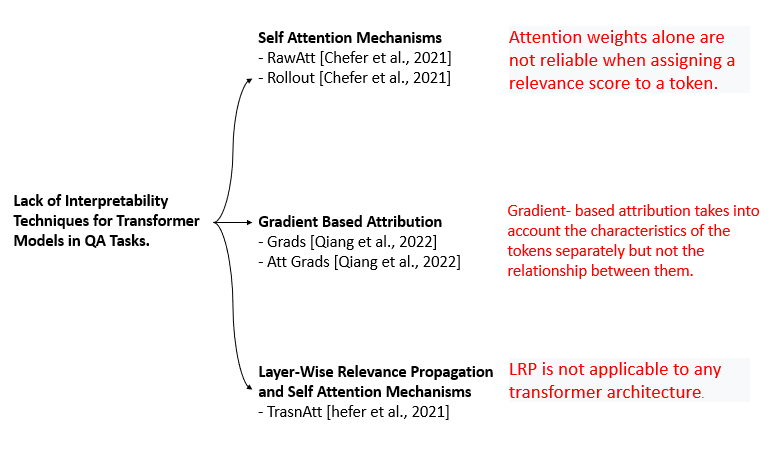
\includegraphics[width=\linewidth]{Figures/Preliminares/SOTA.png}
    \caption{Summary of the-State-of-the-Art Interpretability Techniques for Transformer Models in Question Answering Tasks with its Limitations.}
    \label{fig:sota}
\end{figure}




\subsection{Measures to measure the performance of the interpretability techniques}

\subsubsection{Precision@K}

Inspired by the original Precision@K used in recommender system (\cite{thayaparan2020explanationlp}), \cite{NEURIPS2022_20e45668} designed
a novel Precision@K to evaluate the explanation performance on question answering tasks. For each test example, they count the number of tokens in the answer that appear in the K top-scored tokens as Precision@K. Therefore, higher Precision@K scores are better.


